\chapter{Appendix}
\newpage
\section{lab2}
\subsection{FSM VHDL}
\begin{figure}[!htb]
	\centering
	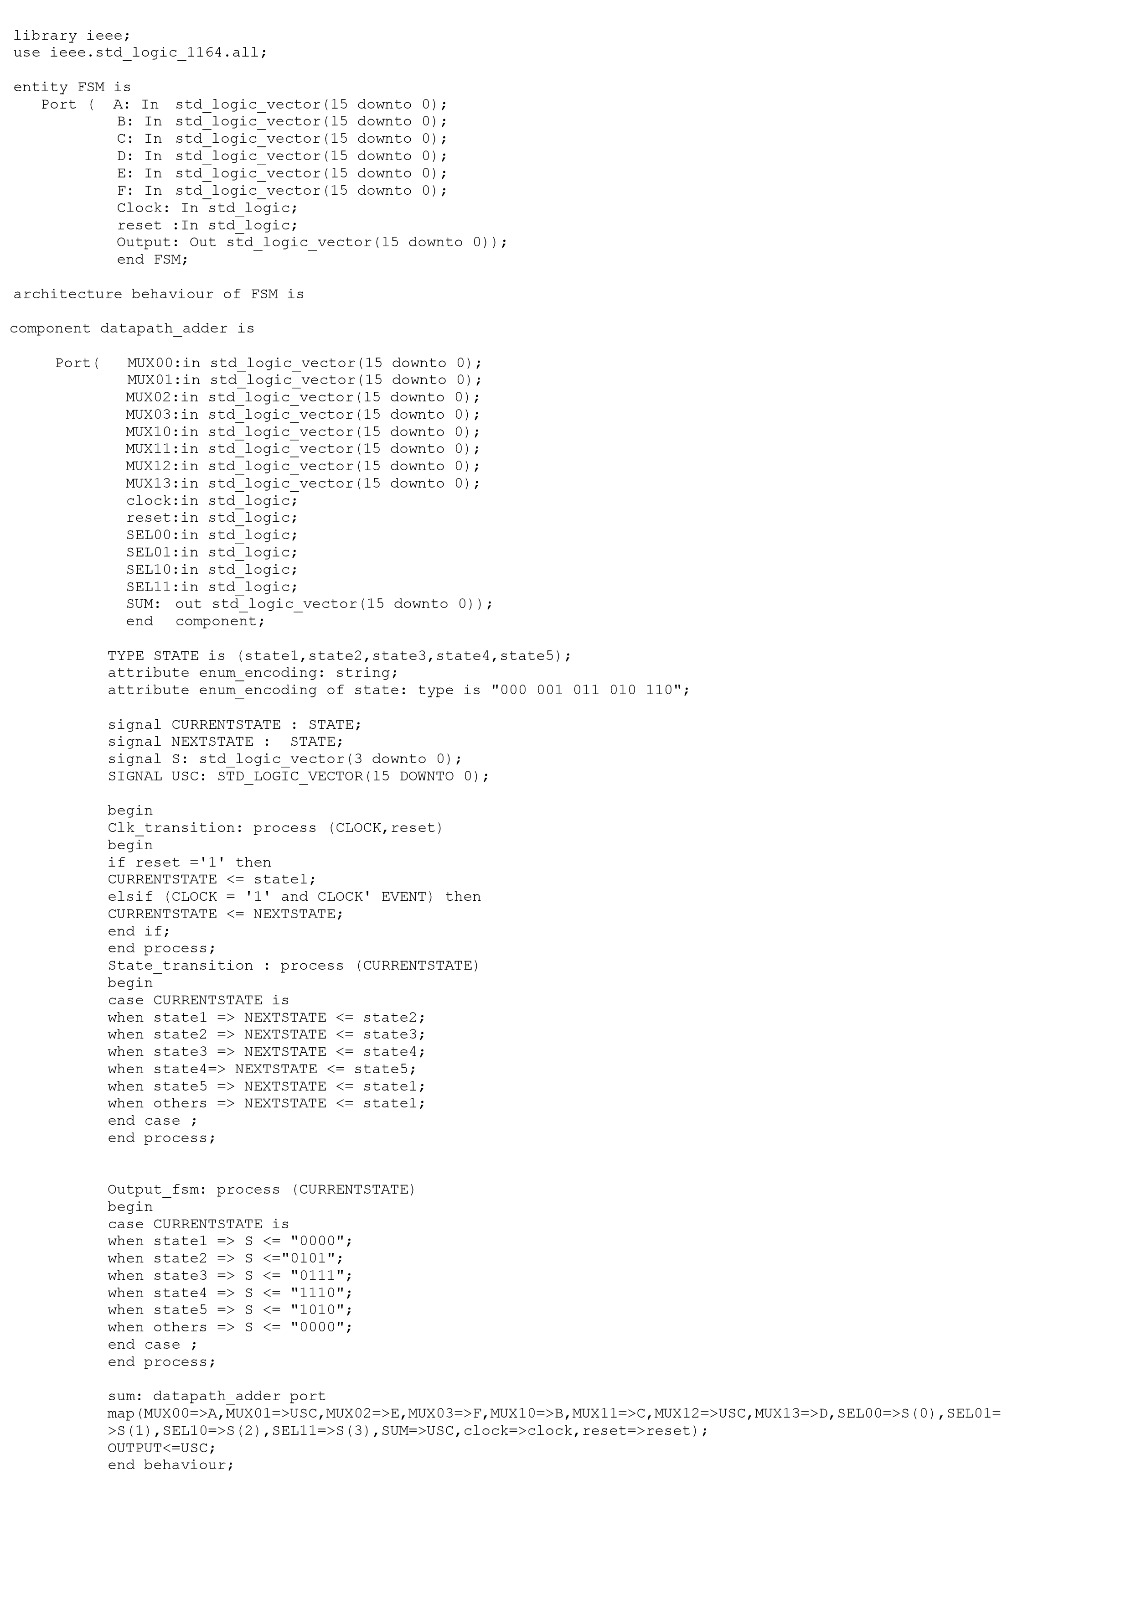
\includegraphics[scale=0.3]{immagini/fsm}
	\caption{\textit{Macchina a stati finiti}}
	\label{fsm}
\end{figure}
\newpage
\section{lab3}
\subsection{CLOCK GATING VHDL}
\begin{figure}[!htb]
	\centering
	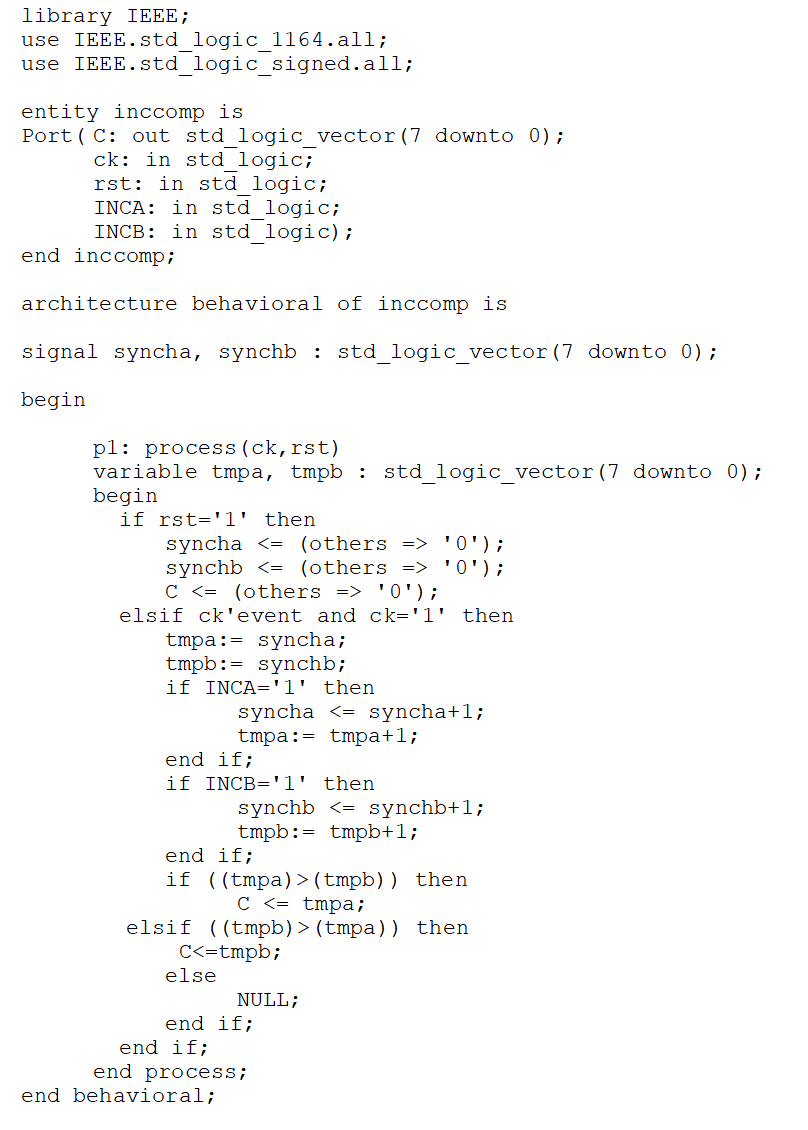
\includegraphics[scale=1]{immagini/3_vhdl}
	\caption{\textit{Schema implementativo della tecnica del Clock Gating}}
	\label{3_vhdl}
\end{figure}
\newpage
\section{lab4}
\subsection{T0 VHDL}
\begin{figure}[!htb]
	\centering
	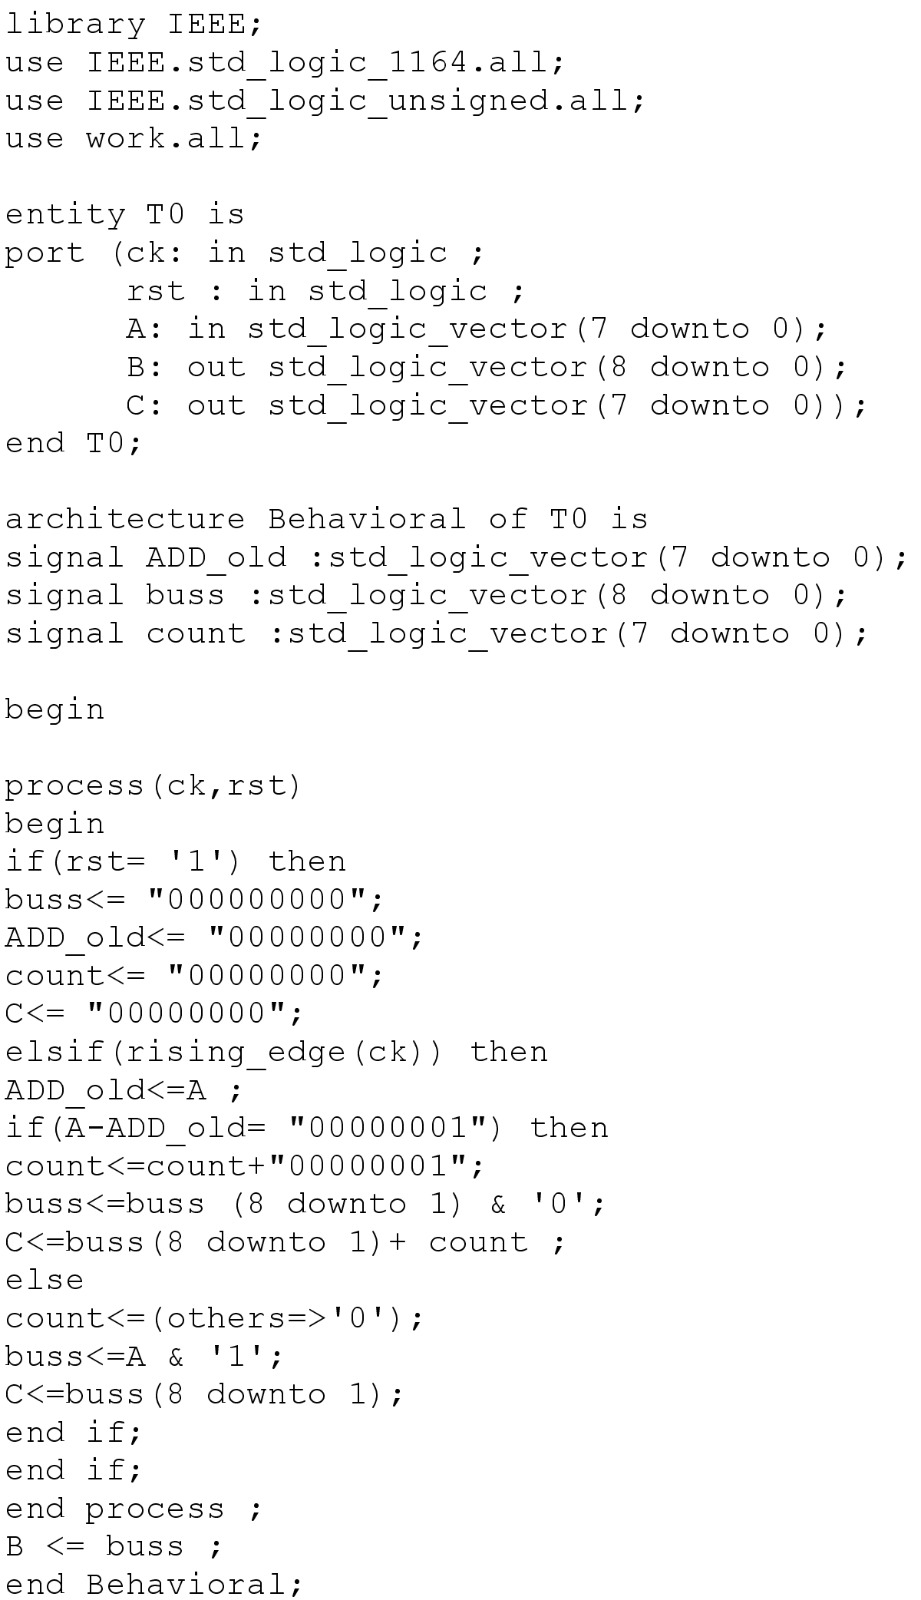
\includegraphics[scale=0.25]{immagini/t0}
	\caption{\textit{Codice codifica T0}}
	\label{t0}
\end{figure}
\newpage
\section{lab6}
\subsection{INCOMP VHDL}
\begin{figure}[!htb]
	\centering
	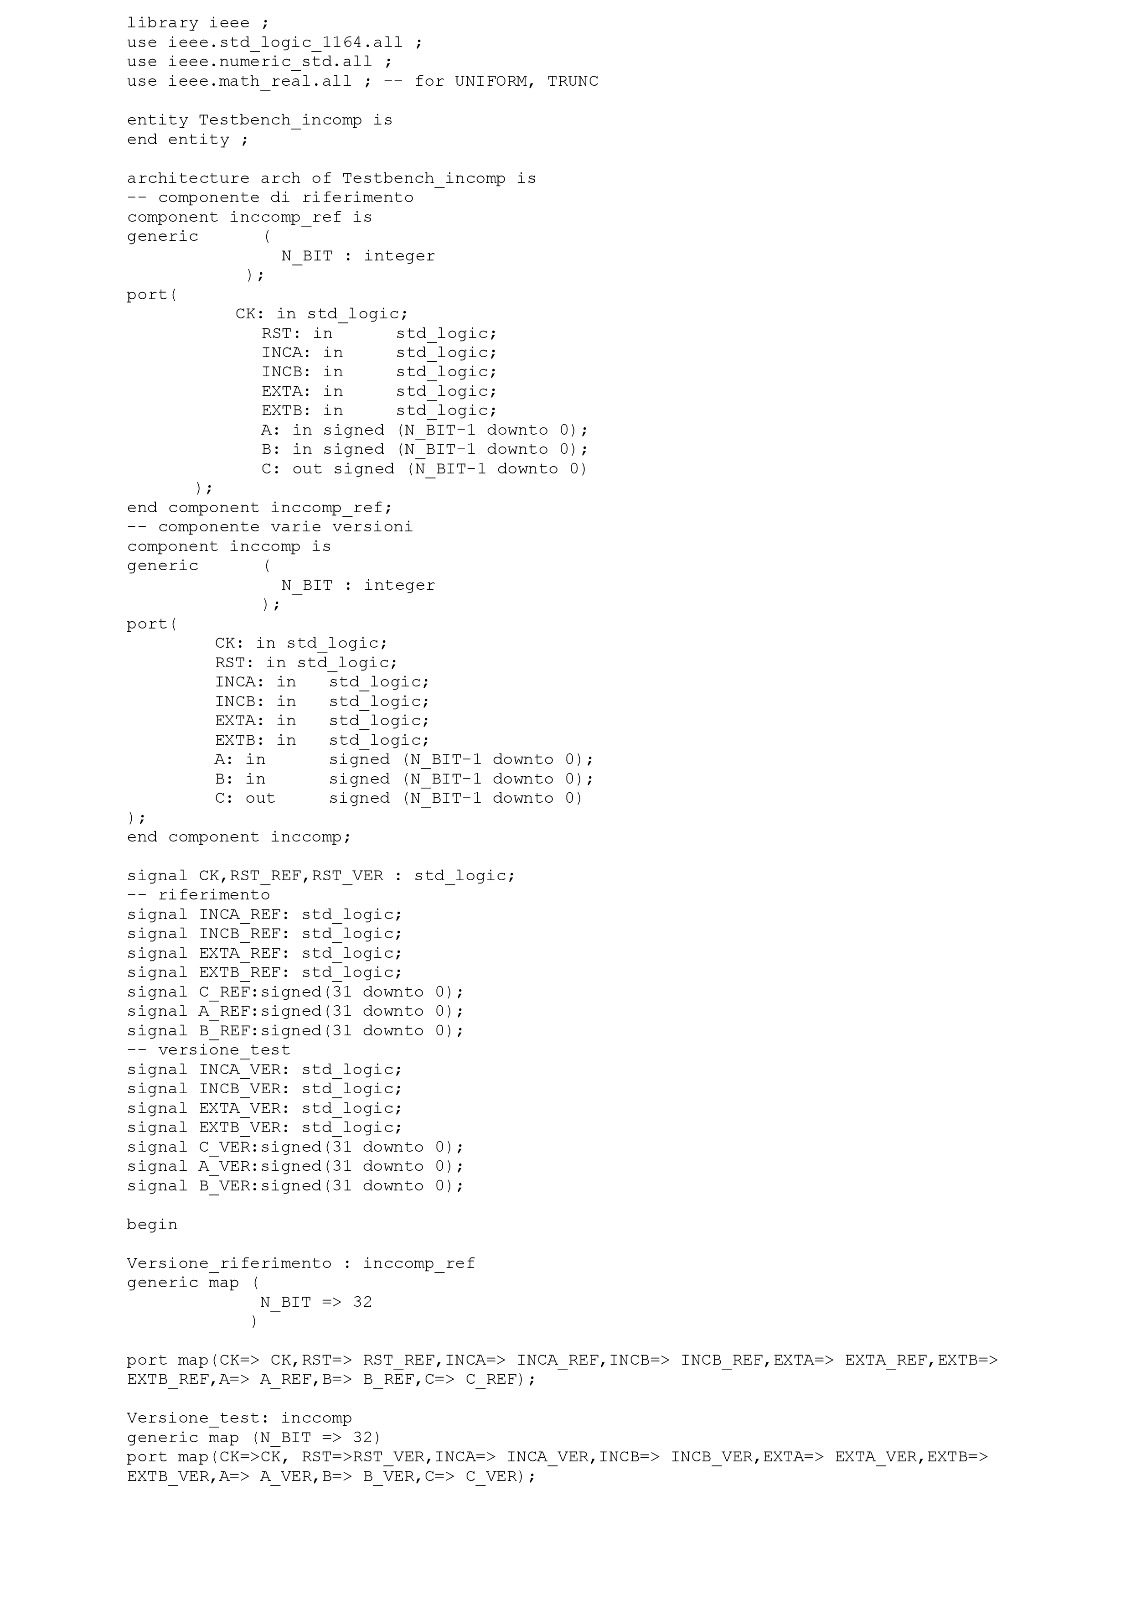
\includegraphics[scale=0.25]{immagini/testbench_vhdl1}
	\label{testbench_vhdl1}
\end{figure}
\begin{figure}[!htb]
	\centering
	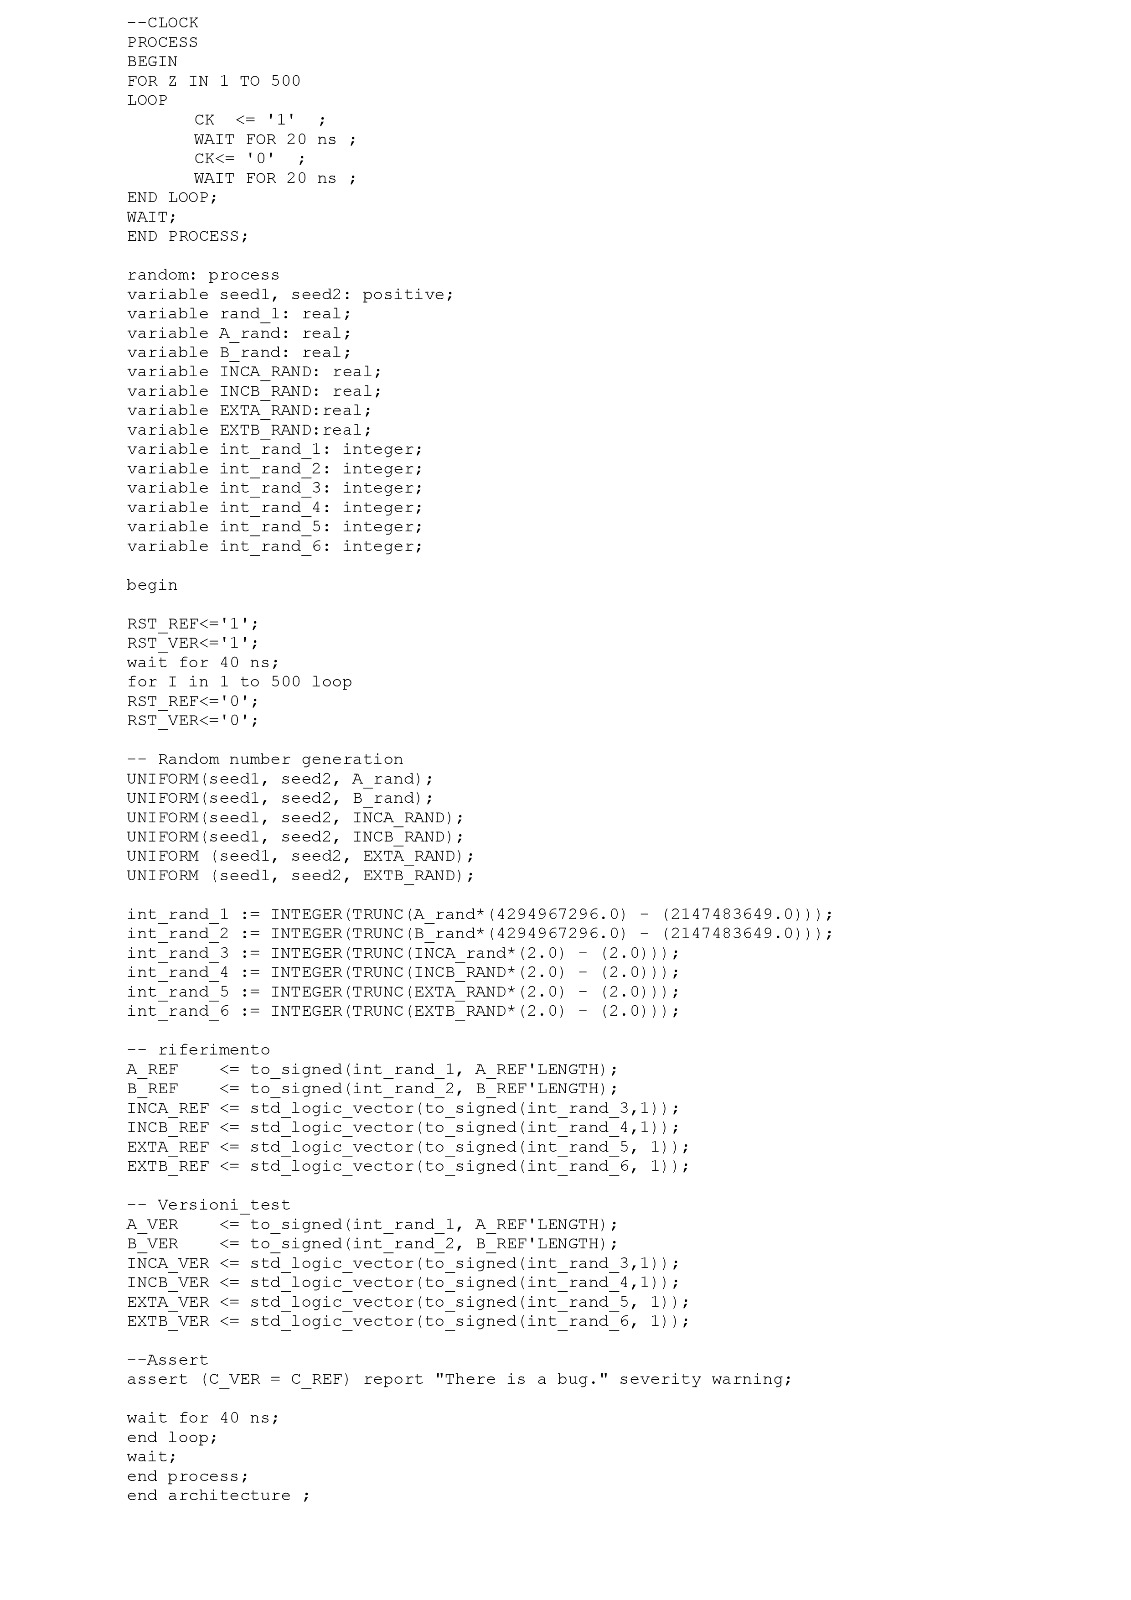
\includegraphics[scale=0.25]{immagini/testbench_vhdl2}
	\caption{\textit{Testbench Incomp}}
	\label{testbench_vhdl2}
\end{figure}
\newpage
\subsection{COUNTER TB VHDL}
\begin{figure}[!htb]
	\centering
	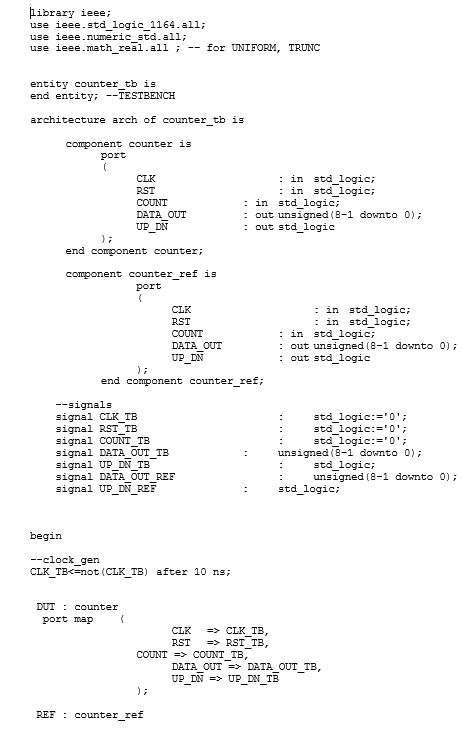
\includegraphics[scale=1.2]{immagini/counter_tb1}
	\label{counter_tb1}
\end{figure}
\begin{figure}[!htb]
	\centering
	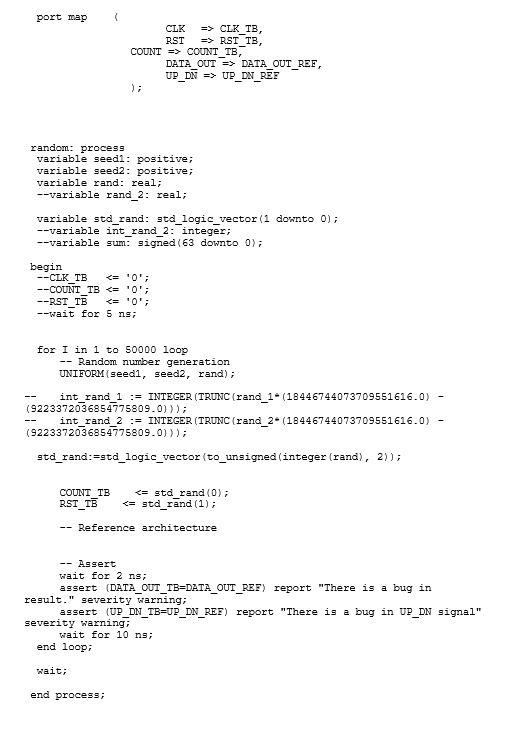
\includegraphics[scale=1.2]{immagini/counter_tb2}
	\label{counter_tb2}
\end{figure}
\begin{figure}[!htb]
	\centering
	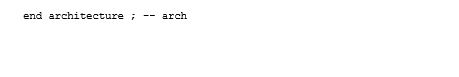
\includegraphics[scale=1.2]{immagini/counter_tb3}
	\caption{\textit{Testbench FSM}}
	\label{counter_tb3}
\end{figure}
\newpage
\subsection{COUNTER TB DO}
\begin{figure}[!htb]
	\centering
	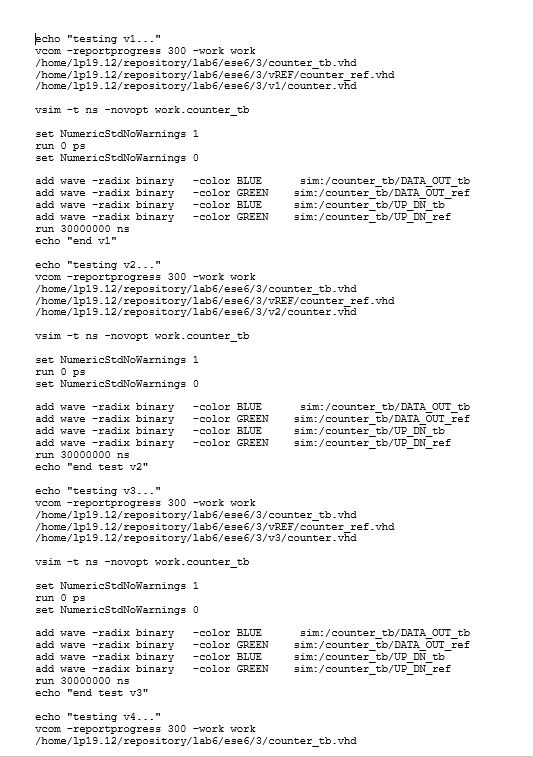
\includegraphics[scale=1.2]{immagini/counterdo1}
	\label{counterdo1}
\end{figure}
\begin{figure}[!htb]
	\centering
	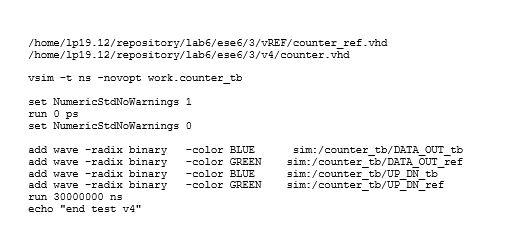
\includegraphics[scale=1.2]{immagini/counterdo2}
	\caption{\textit{Script di comando Modelsim}}
	\label{counterdo2}
\end{figure}
\newpage
\subsection{TESTING SCRIPT PY}
\begin{figure}[!htb]
	\centering
	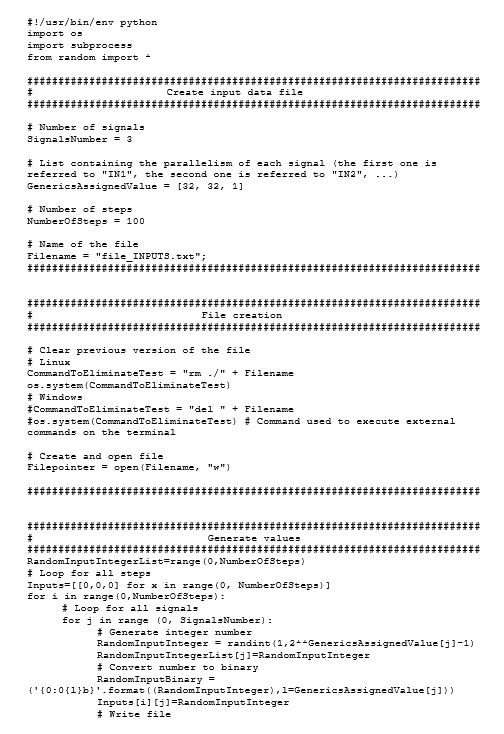
\includegraphics[scale=1.2]{immagini/testing1}
	\label{testing1}
\end{figure}
\begin{figure}[!htb]
	\centering
	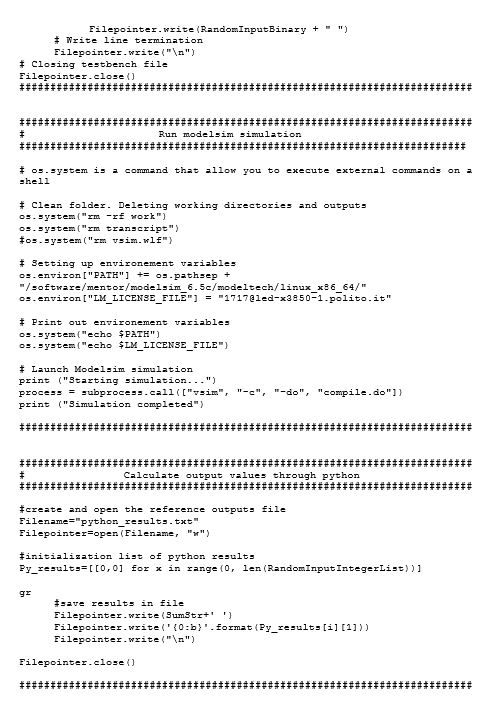
\includegraphics[scale=1.2]{immagini/testing2}
	\caption{\textit{Script file di testing completo}}
	\label{testing2}
\end{figure}
\newpage
\subsection{TB GENERATOR PY}
\begin{figure}[!htb]
	\centering
	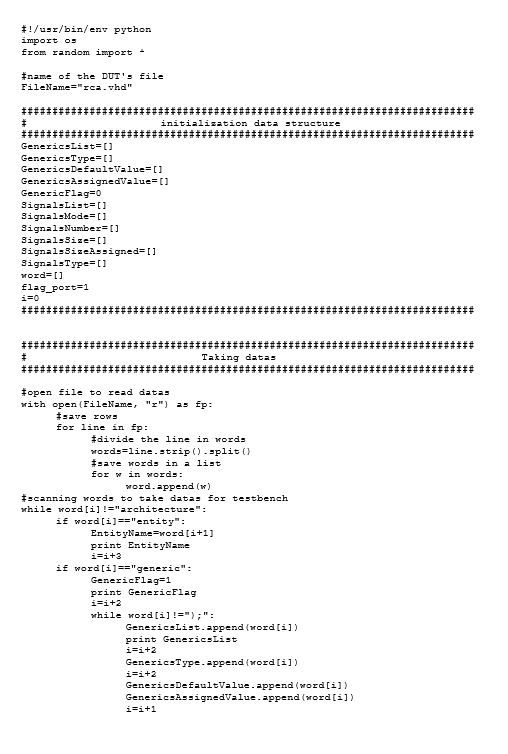
\includegraphics[scale=1.2]{immagini/tbgen1}
	\label{tbgen1}
\end{figure}
\begin{figure}[!htb]
	\centering
	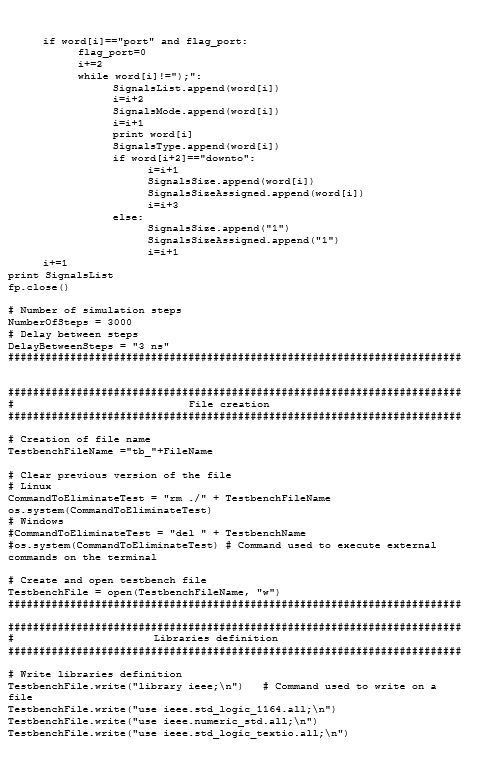
\includegraphics[scale=1.2]{immagini/tbgen2}
	\label{tbgen2}
\end{figure}
\begin{figure}[!htb]
	\centering
	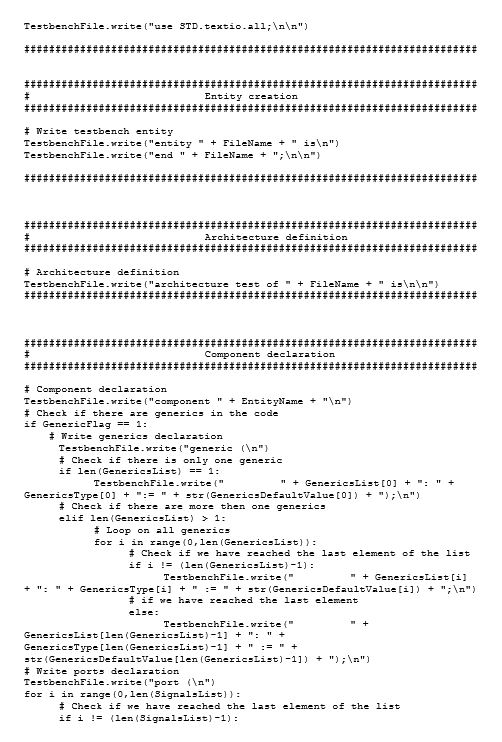
\includegraphics[scale=1.2]{immagini/tbgen3}
	\label{tbgen3}
\end{figure}
\begin{figure}[!htb]
	\centering
	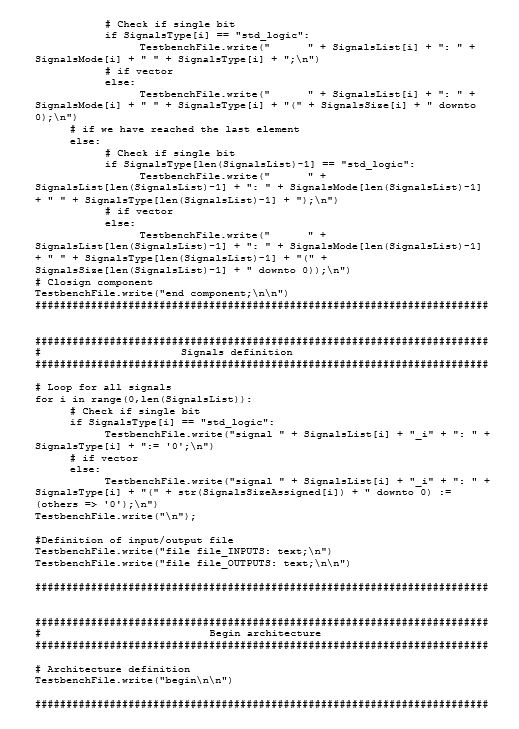
\includegraphics[scale=1.2]{immagini/tbgen4}
	\caption{\textit{Script file di testing completo}}
	\label{tbgen4}
\end{figure}
\begin{figure}[!htb]
	\centering
	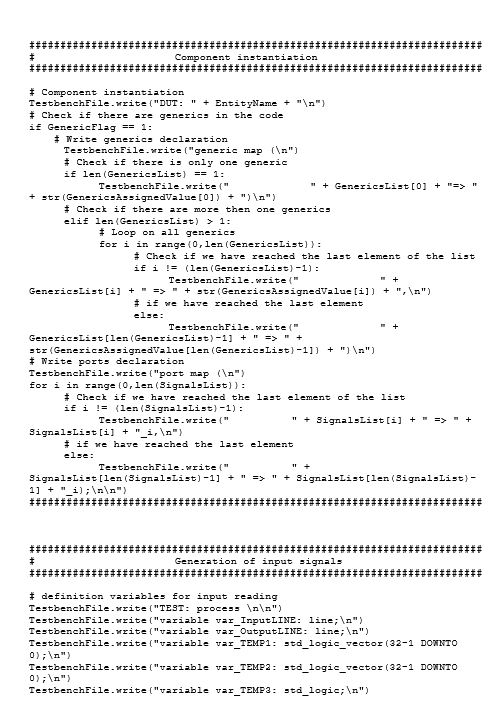
\includegraphics[scale=1.2]{immagini/tbgen5}
	\label{tbgen5}
\end{figure}
\begin{figure}[!htb]
	\centering
	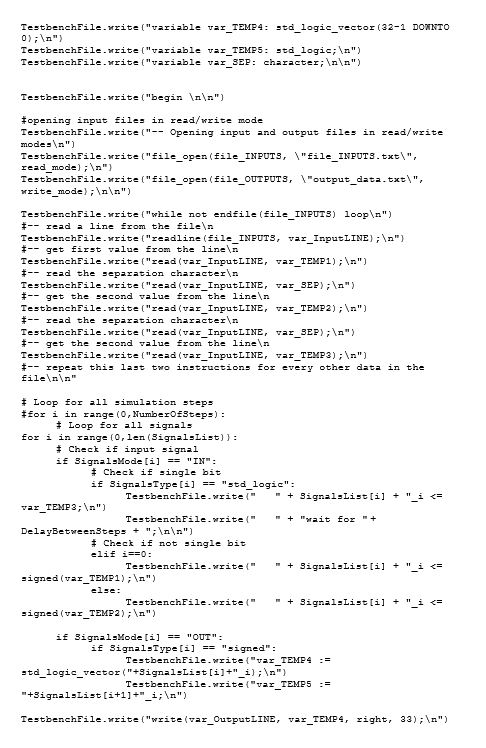
\includegraphics[scale=1.2]{immagini/tbgen6}
	\label{tbgen6}
\end{figure}
\begin{figure}[!htb]
	\centering
	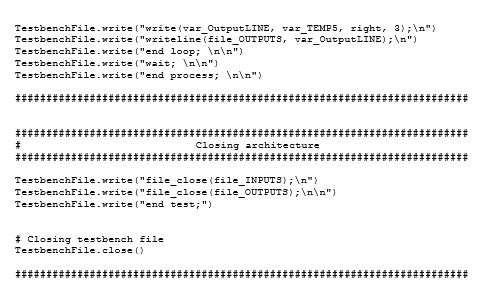
\includegraphics[scale=1.2]{immagini/tbgen7}
	\caption{\textit{Python file di creazione testbench}}
	\label{tbgen7}
\end{figure}